\section{Results}

\subsection{Topic Selection}

\begin{figure}[H]
    \centering
    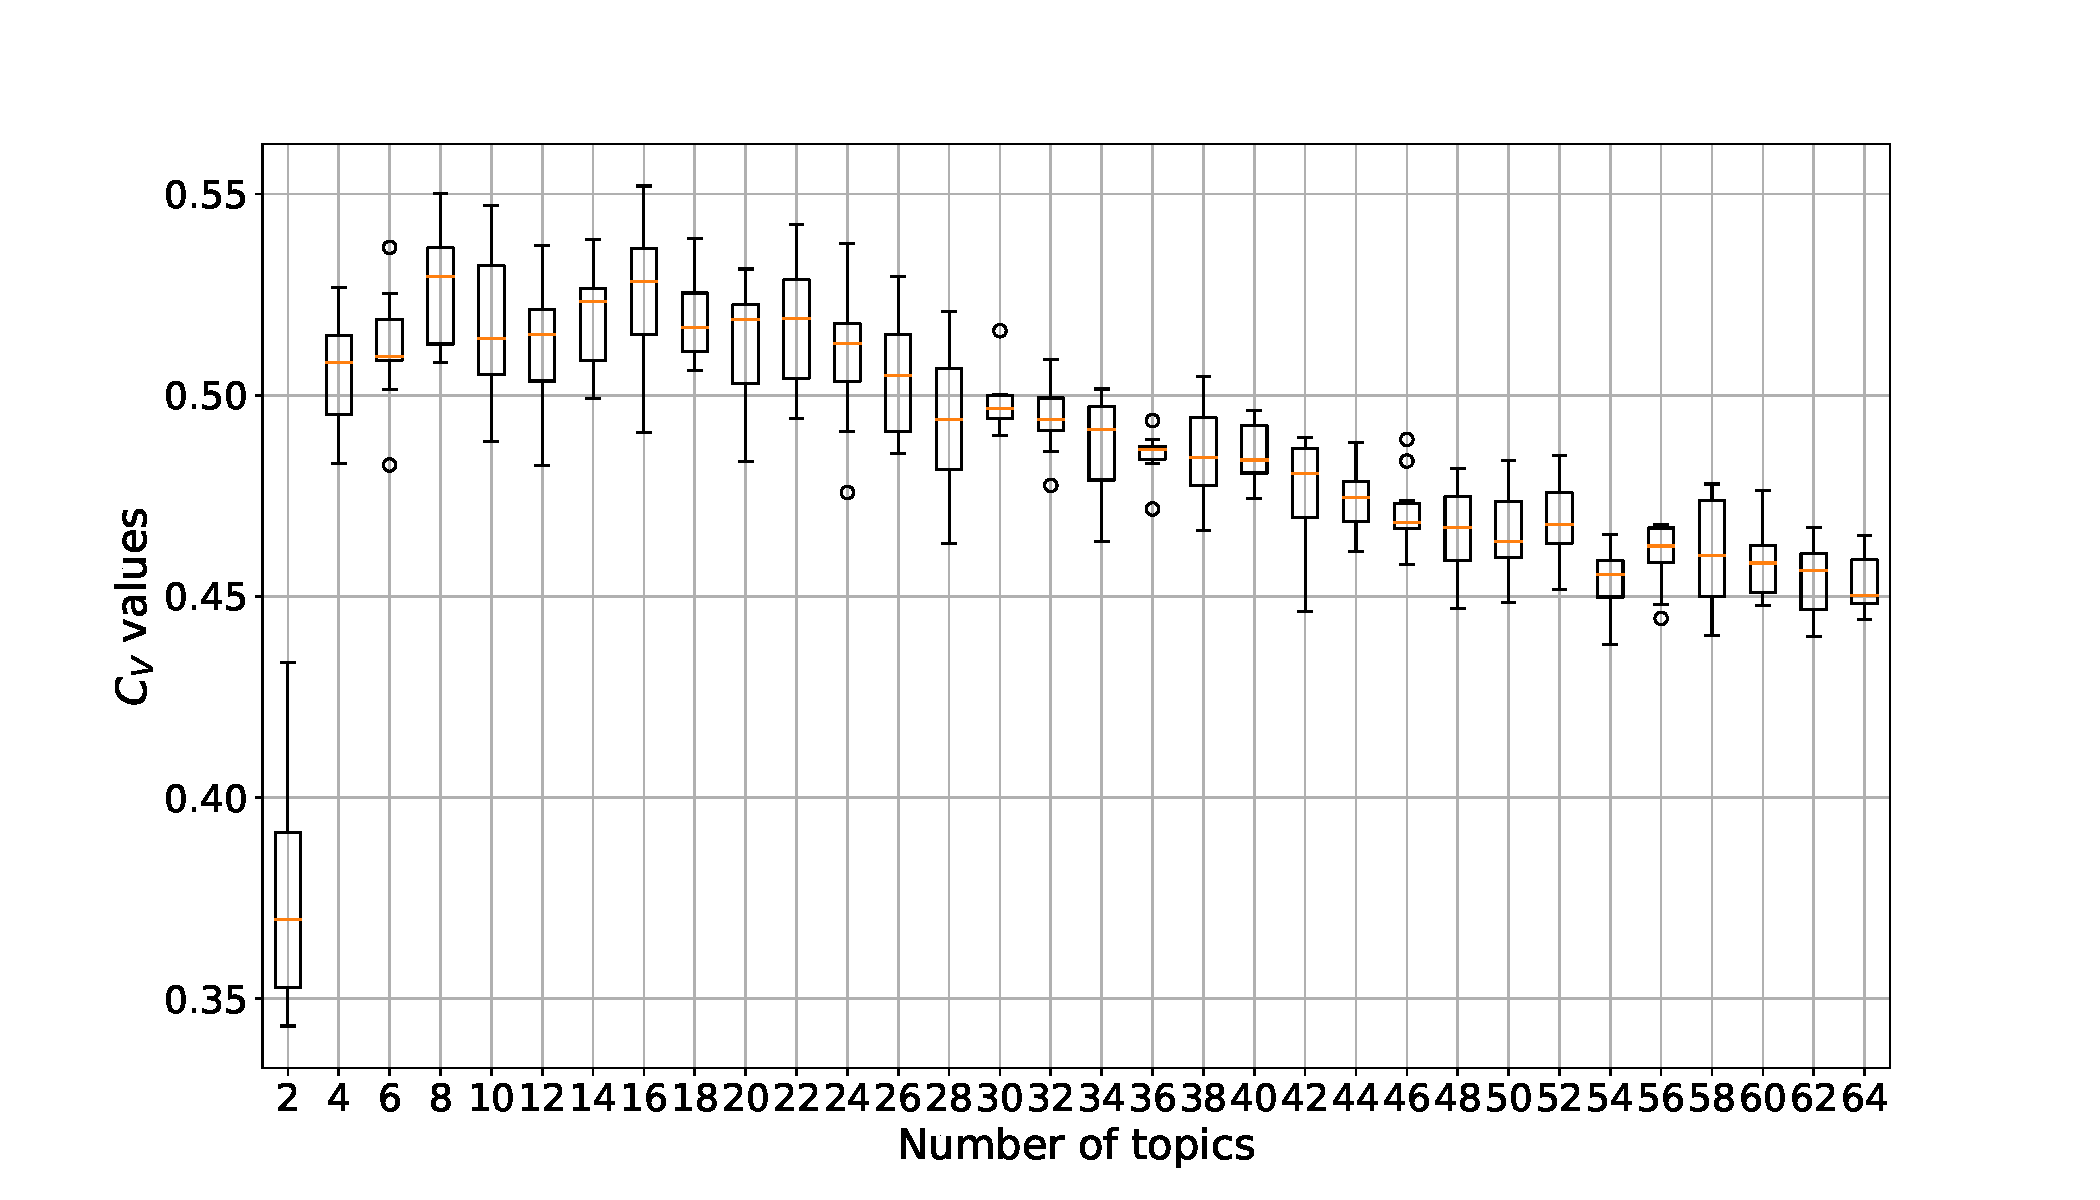
\includegraphics[width = 16cm, height = 8cm]{Code/img/topic_selection.pdf}
    \caption[The result of the coherence measurement]{\textbf{Coherence measurement:} The figure shows the result of the coherence measure ($C_v$) for topic models with 2 to 64 topics with increment by 2, every observation is the boxplot of coherence vector of each k-topic model. The orange line of every boxplot represents the median $C_v$ value of each 10-run LDA model with given topics. Higher median $C_v$ values are preferred.}
\end{figure}

Fig 1 shows an increase in $C_v$ values from 2 and 8 topics, while a decreasing trend occurred from 22 to 64 topics. Therefore, the topic models with 8 to 22 topics (8 topic models in total) were selected for the $stability$ test since their median $C_v$ values are significantly higher than others, where the 8-topic models have maximum median $C_v$ value (Median $C_v = 0.53$) and 10-topic models have minimum median $C_v$ value (Median $C_v = 0.51$).

\begin{figure}[H]
    \centering
    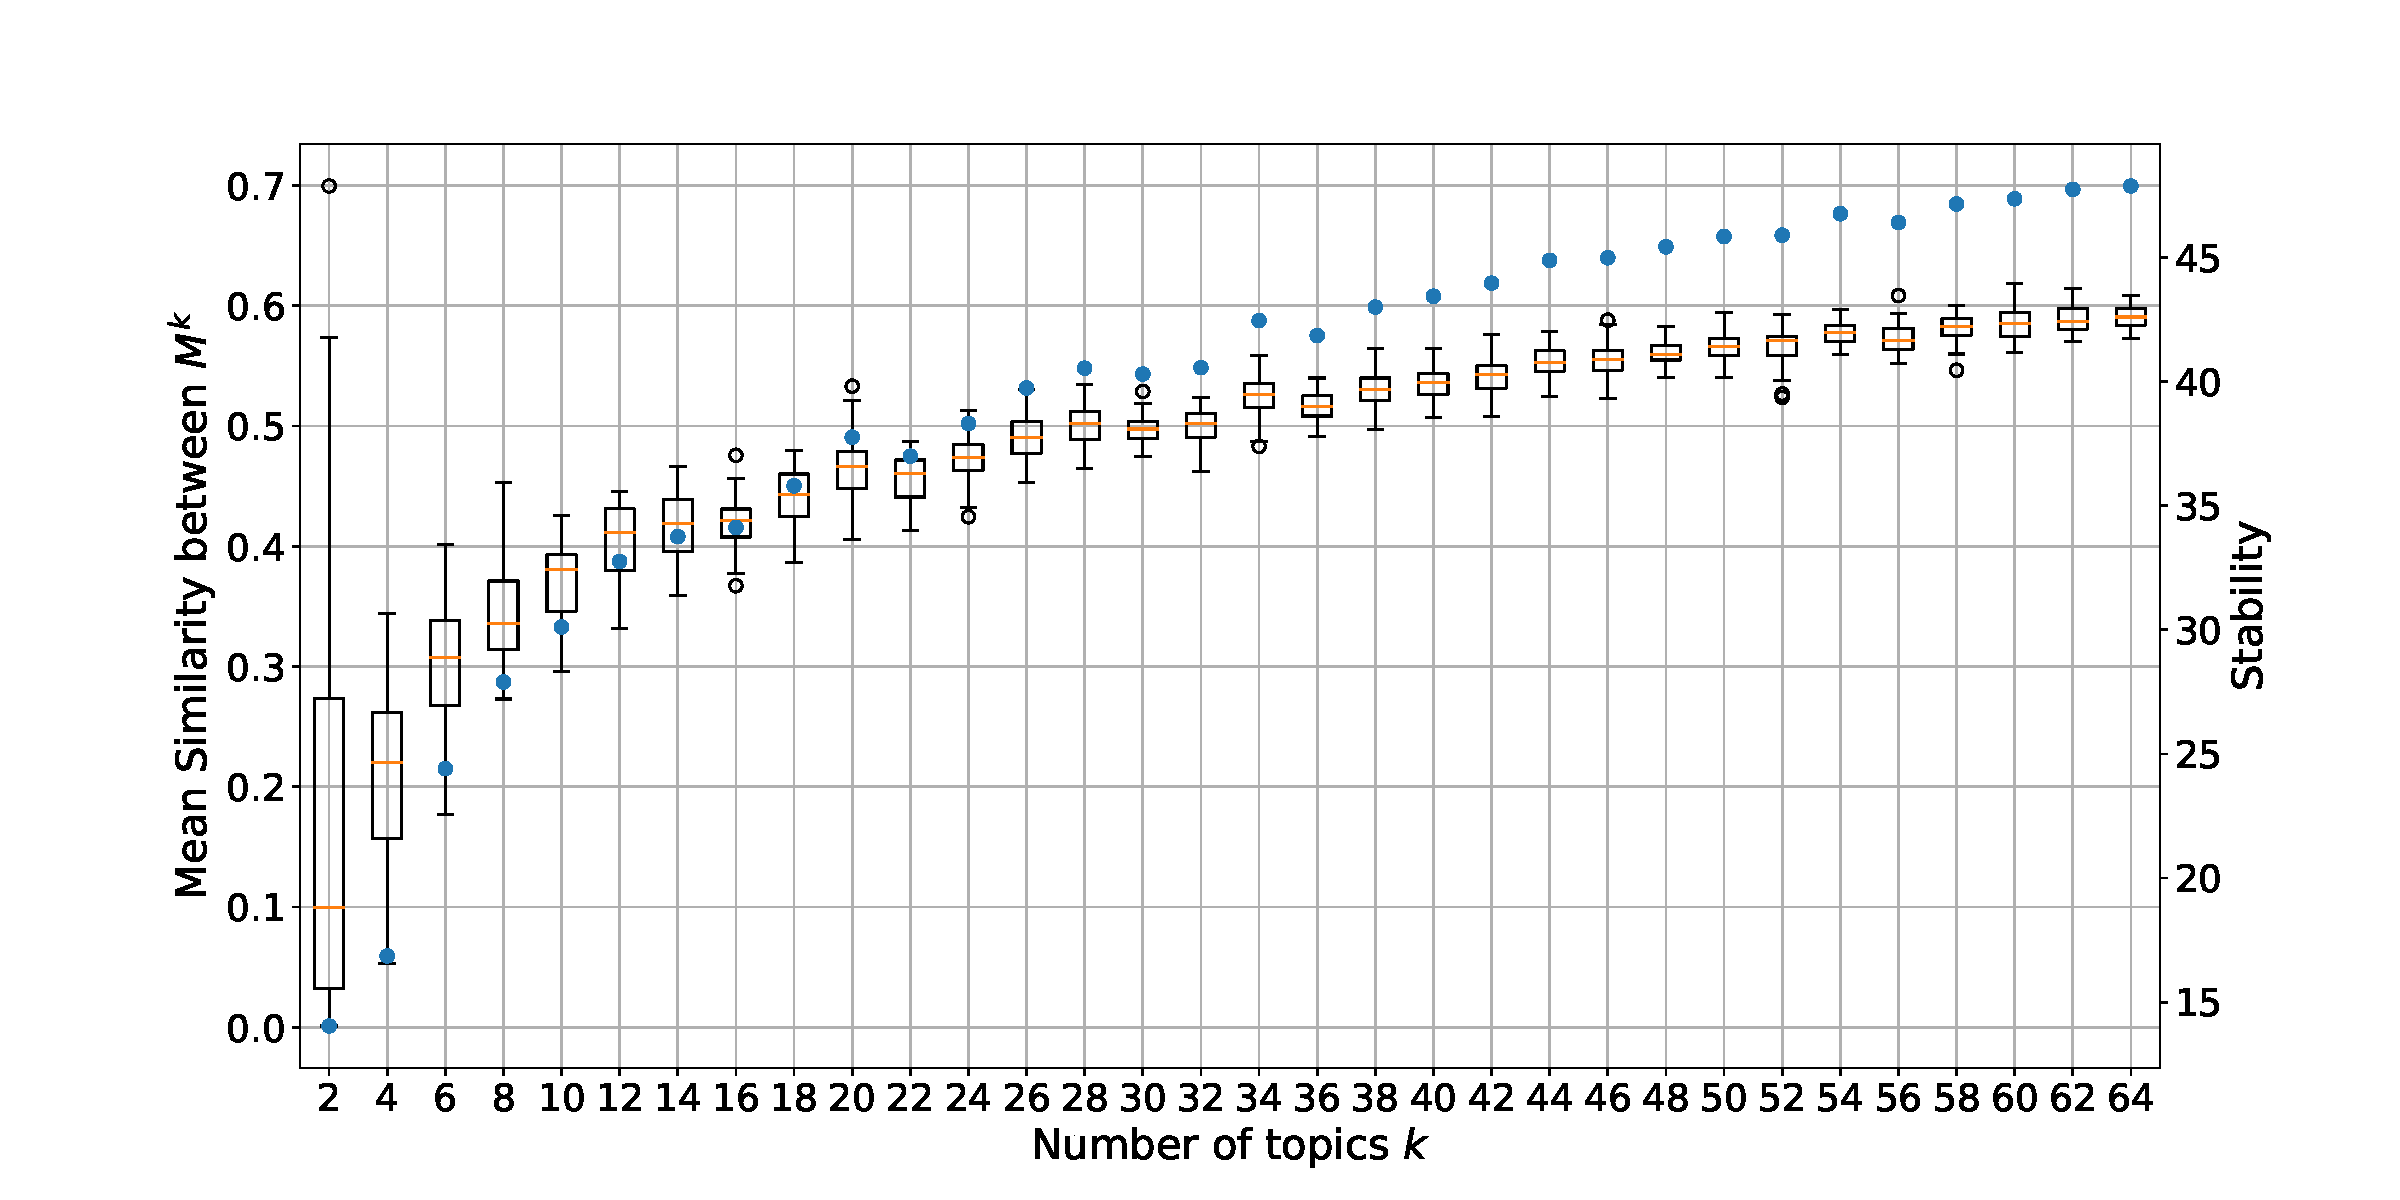
\includegraphics[width = 16cm, height = 8cm]{Code/img/jsd_boxplot.pdf}
    \caption[Mean similarity and stability between models]{\textbf{Mean similarity and stability between models}: The main y-axis is the averaged $similarity$. Each boxplot is a vector of averaged $similarity$ values. The secondary y-axis represents $stability$ values, which are blue points in the figure. The best model should have the lowest mean $similarity$ and $stability$ values (see Support Information section) in the subset of k-topic models selected by $C_v$ metrics.}
\end{figure}

Furthermore, the averaged $similarity$ and model $stability$ both show an increasing trend from topic 2 to topic 64 in general. The 8-topic model has the lowest median averaged $similarity$ (median $Sim(M^k) = 0.34$) and $stability$ ($Stab(M^k) = 27.9$) between eight models selected by coherence measurement. In conclusion, by figures above, the 8-topic LDA model has the highest median $C_v$ value while its median mean $similarity$ and $stability$ values are also lowest compared to other selected topic models. Therefore, the 8-topic LDA model is considered as the final model throughout the analysis.

\subsection{LDA Model Fitting and Topic Visualisation}

\begin{figure}[H]
    \centering
    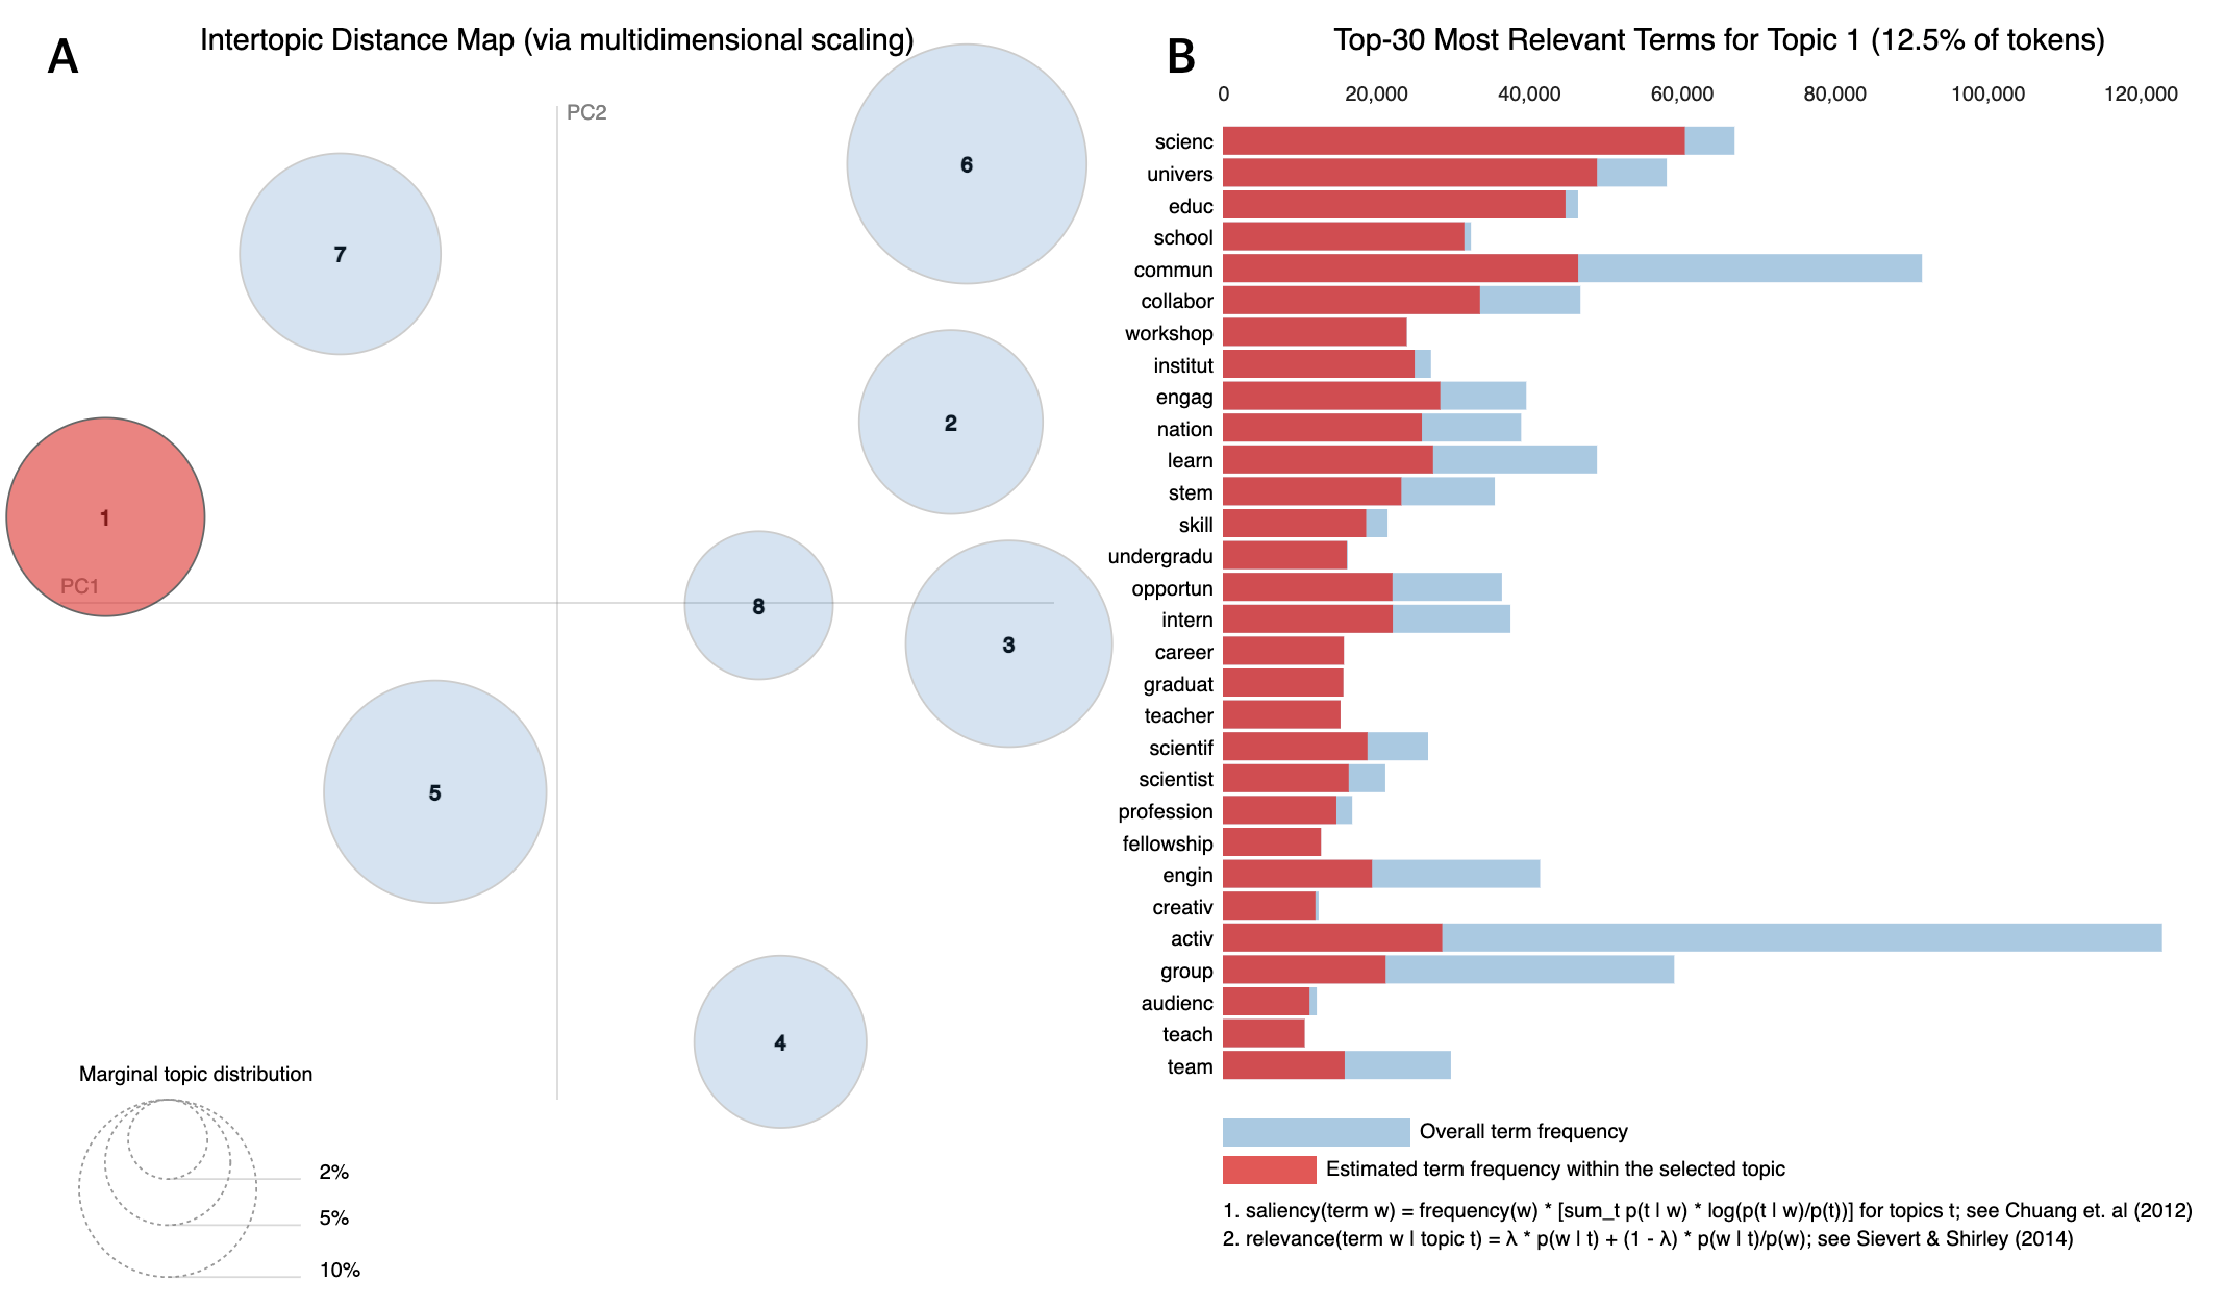
\includegraphics[width = 16cm, height = 9cm]{Code/img/LDAvis.pdf}
    \caption[Interactive visualisation for topic distributions]{\textbf{Topic Visualisation:} An example of interactive visualisation for topic 1 produced from the 8-topic LDA model. Figure A projects eight topics onto a two-dimensional plane by Principal Component Analysis (PCA), where centres of topic circles represent the distance between topics. The areas of circles represent the frequency of topics. Figure B provides a bar chart, where red bars are the frequency of the most relevant stemmed words in topic 1, light blue bars show the corpus-wide word frequency of the individual topic words.}
\end{figure}

For the interpretability of topics, $\lambda$ is adjusted to 0.61 (see Support Information section). From Fig.3 A, there is no overlap between the areas of 8 topics, indicating that 8 topics are well-distributed on the two-dimensional plane, supporting that the topic model with 8 topics could be the best-fit model in my dataset. For Fig.3 B, the most five relevant words are `science’, `university’, `education’, `school’ and `collaboration’ respectively. Thus, the first topic might be relevant with ``Higher Education”. I used the same logic to assign labels for all eight topics. The labels of eight topics are: ``Higher Education", ``Brain Science", ``Protein Chemistry and Microbiology", ``Material Science and Physics", ``Computer System and Commercial Application", ``Cancer Treatment and Immunology", ``Social Policy and Public Healthcare" and ``Climate Change and Environment".

\begin{figure}[H]
    \centering
    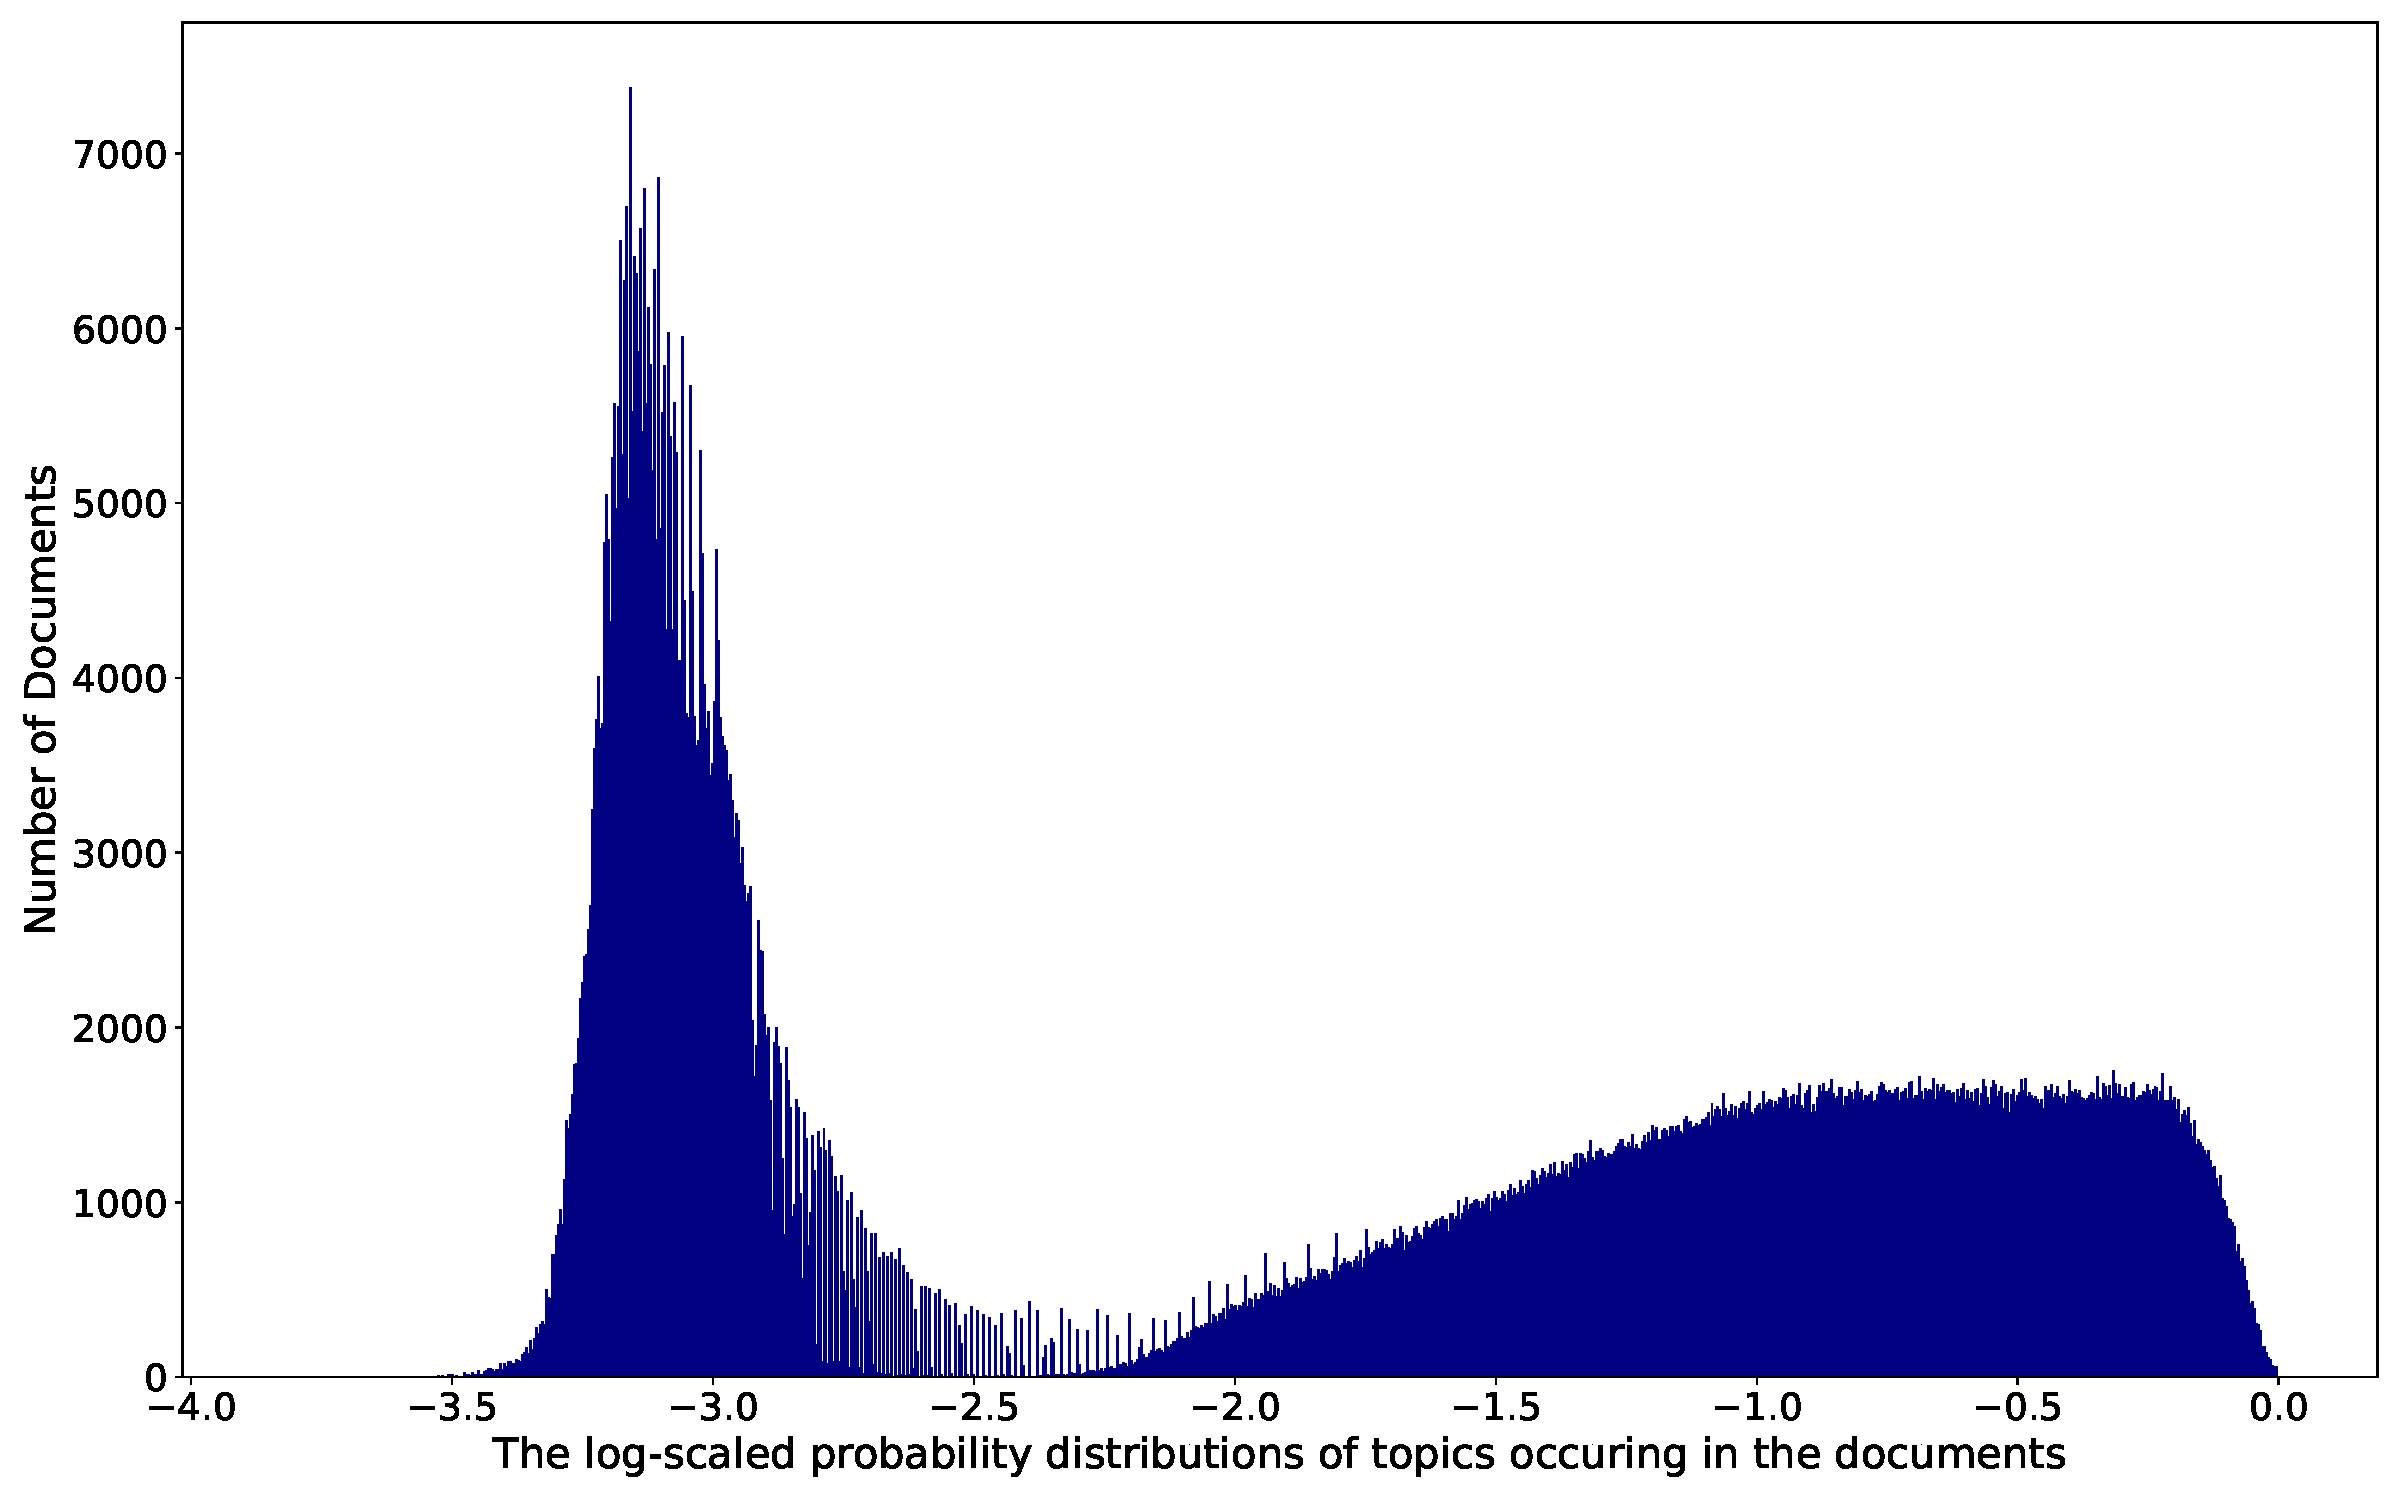
\includegraphics[width = 14cm, height = 8cm]{Code/img/distri_doc_word_counts.pdf}
    \caption[Probability distributions of all topics from all documents]{\textbf{Topic Distribution:} The figure shows log-scaled (with base 10) probability distributions of all topics from all documents.}
\end{figure}

The probability distribution of topics in each document might not always be helpful for topic identification since all topics can have non-zero probabilities occurring in each document \cite{LDA}, indicating that the probabilities for some topics are too small to be informative. Therefore, I plotted the topic probabilities throughout documents based on base 10 logarithm. Two peaks can be seen in Fig. 3, where one occurred as the probabilities are between $10^{-3.5}$ and $10^{-2.5}$, another peak is distributed from approximately $10^{-1}$ to $10^{-0.2}$. Hence, in order to remove all uninformative topics for each topic, any topics of which the probability is less than the minima between two peaks, at $10^{-2.3}$ (i.e. 0.005), are ignored.

\begin{figure}[H]
    \centering
    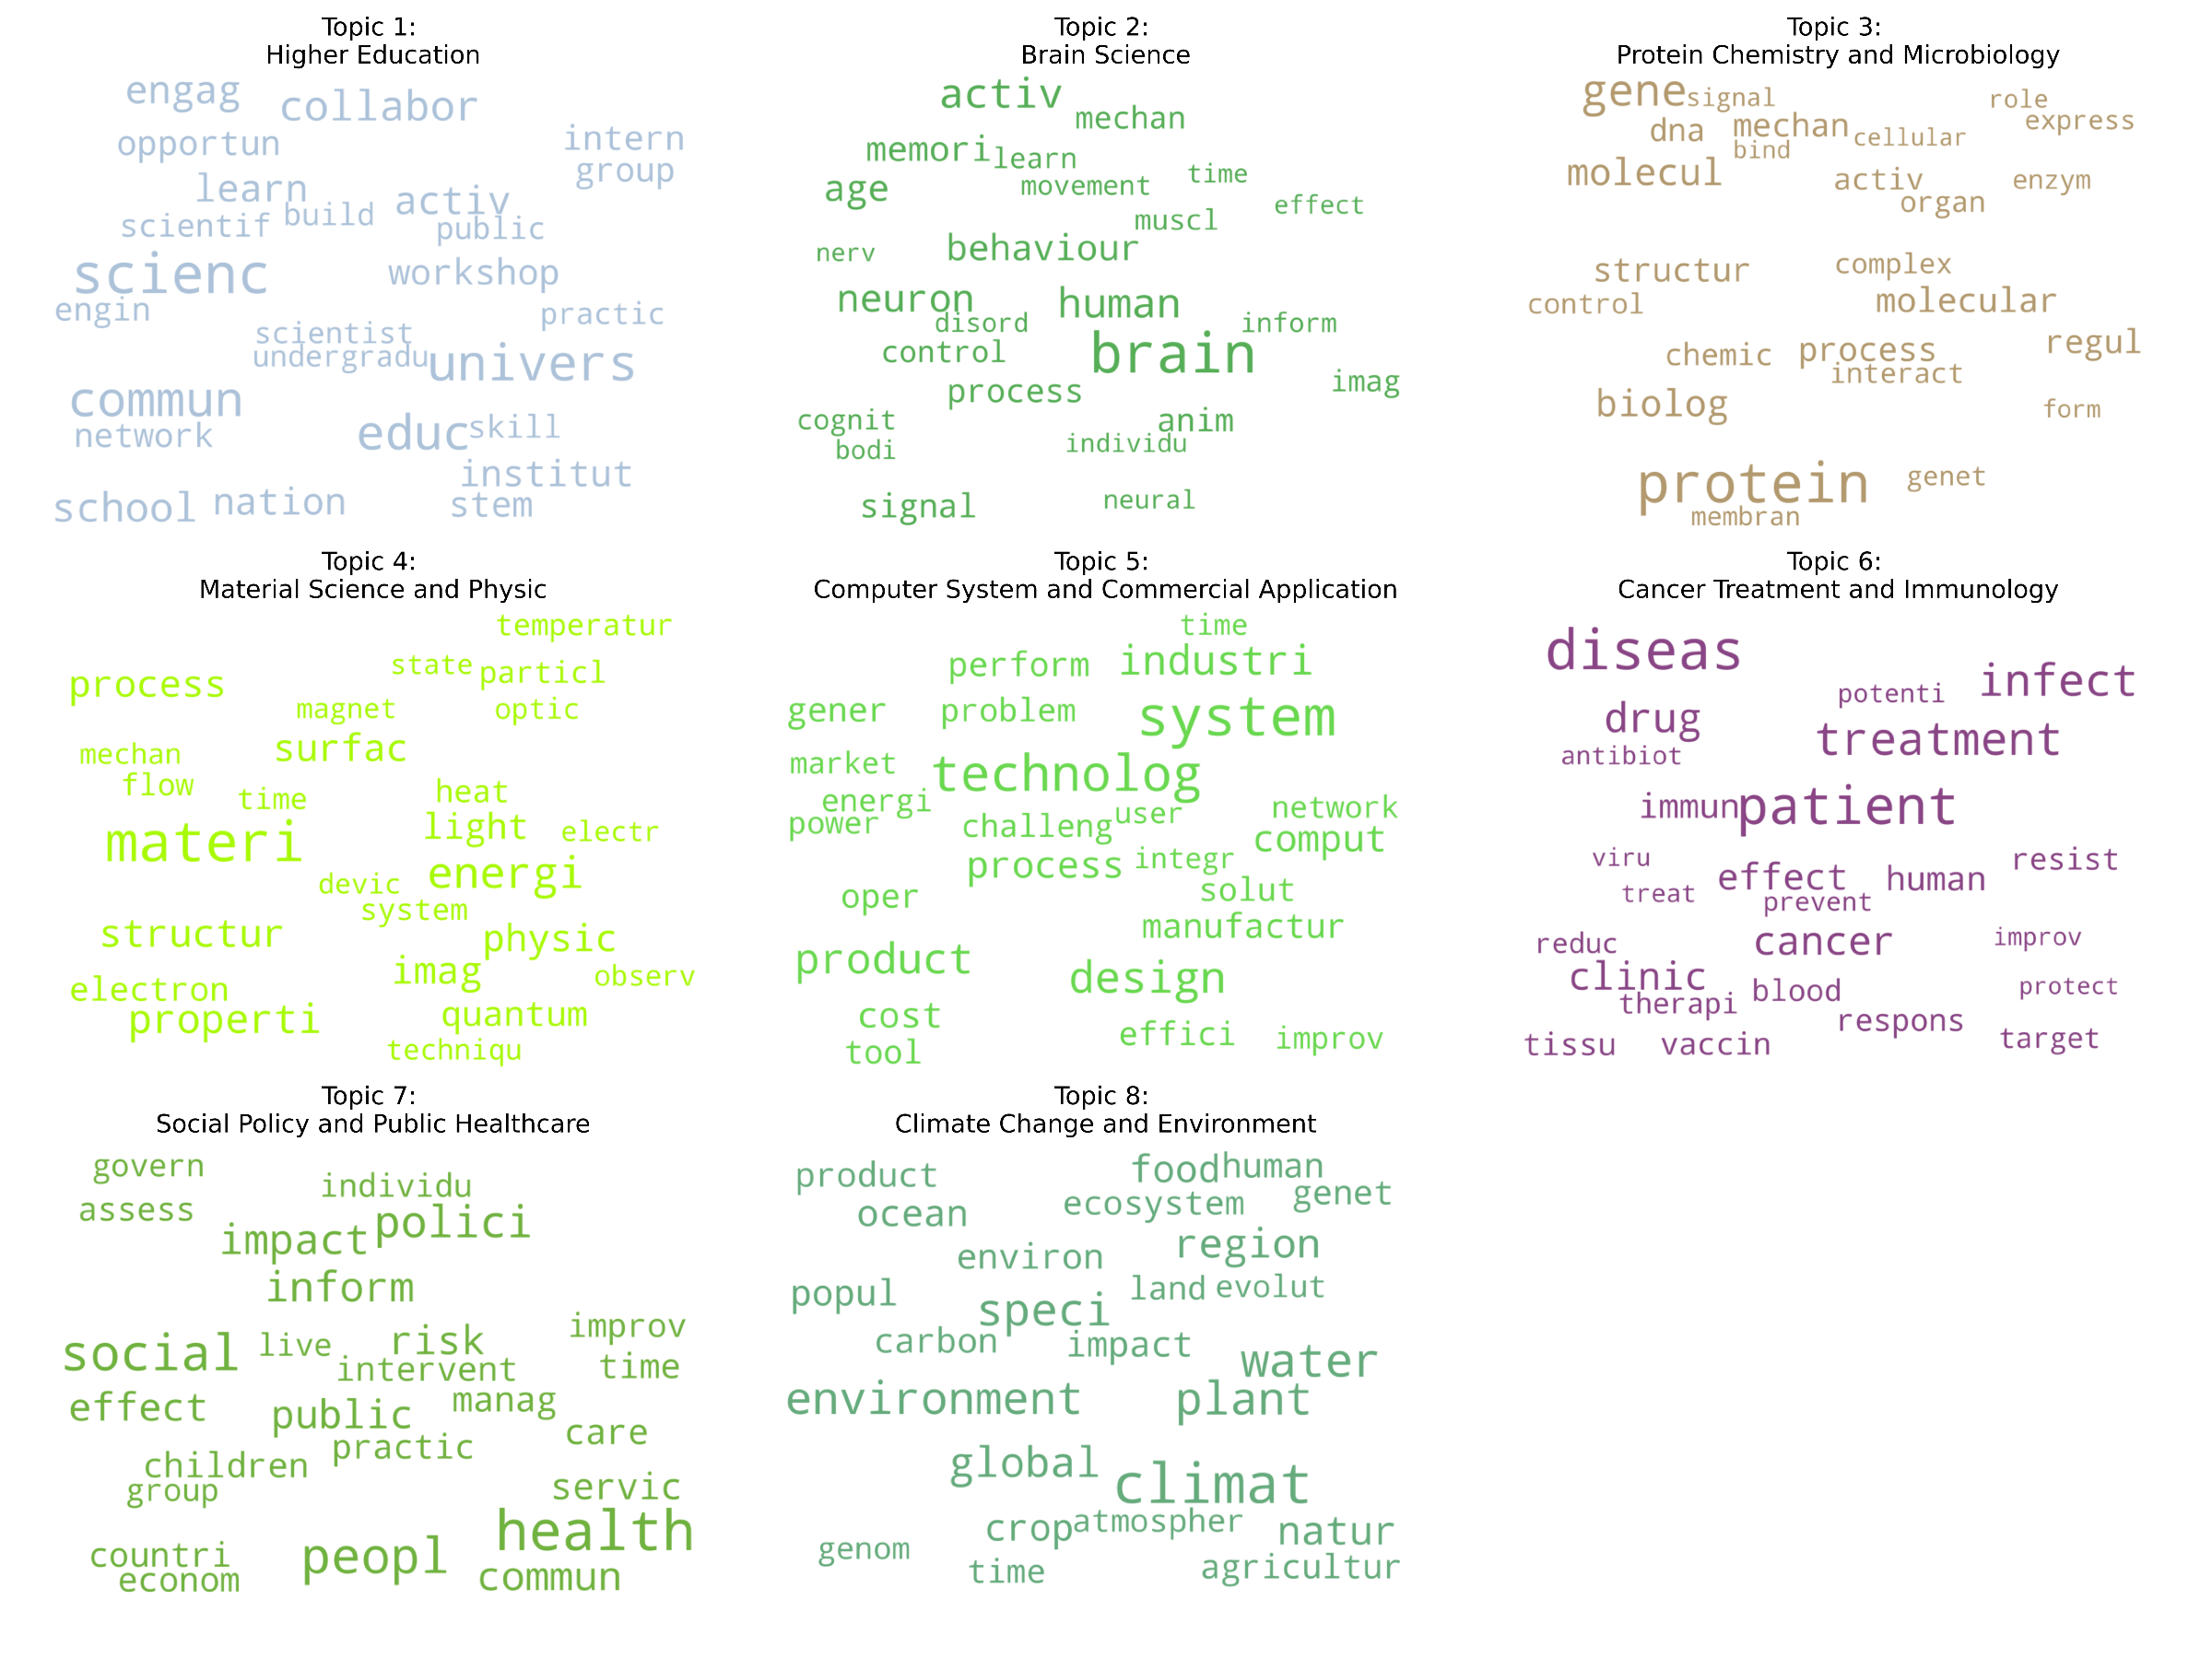
\includegraphics[width = 16cm, height = 11cm]{Code/img/keywords_word_cloud.pdf}
    \caption[Eight wordclouds of top 25 stemmed words]{\textbf{Topic Wordclouds:} The figure shows the wordclouds including top 25 stemmed words of each topic derived from the LDA model, titles for the wordclouds are topic labels assigned manually.}
\end{figure}

\subsection{Topic Analysis}

In general, excluding the ``Higher Education" Topic in ERC, the topic occurrence probabilities of topic 5 (Computer System and Commercial Application), topic 4 (Material Science and Physics) and topic 1 (Higher Education) are relatively high in NSF, ERC and UKRI, whereas other topics occurred relatively more rarely. For NIH agency, ``Cancer Treatment and Immunology" (topic 6), ``Protein Chemistry and Microbiology" (topic 3), ``Brain Science" (topic 2),  and ``Social Policy and Public Healthcare" (topic 7) have higher mean topic probabilities in total, which is not surprising as NIH is a funding agency mainly focusing on medical and health-related research, supporting that my LDA model can obtain topic distributions for projects accurately.

For the group of all other agencies (Fig. 6), they are all dominated by ``Computer System and Commercial Application" with the mean probability approximately $10^{-0.56}$, $10^{-0.61}$ and $10^{-0.54}$ in NSF, ERC and UKRI respectively. For the agency NIH, it is dominated by ``Cancer Treatment and Immunology" whose mean probability is $10^{-0.53}$. Moreover, the ``Climate Change and Environment" and ``Brain Science" topics are prevalent (i.e. larger than or equal to $10^{-1}$) solely in NSF and NIH respectively, whereas other topics are prevalent in 2 agencies at least.

\begin{figure}[H]
    \centering
    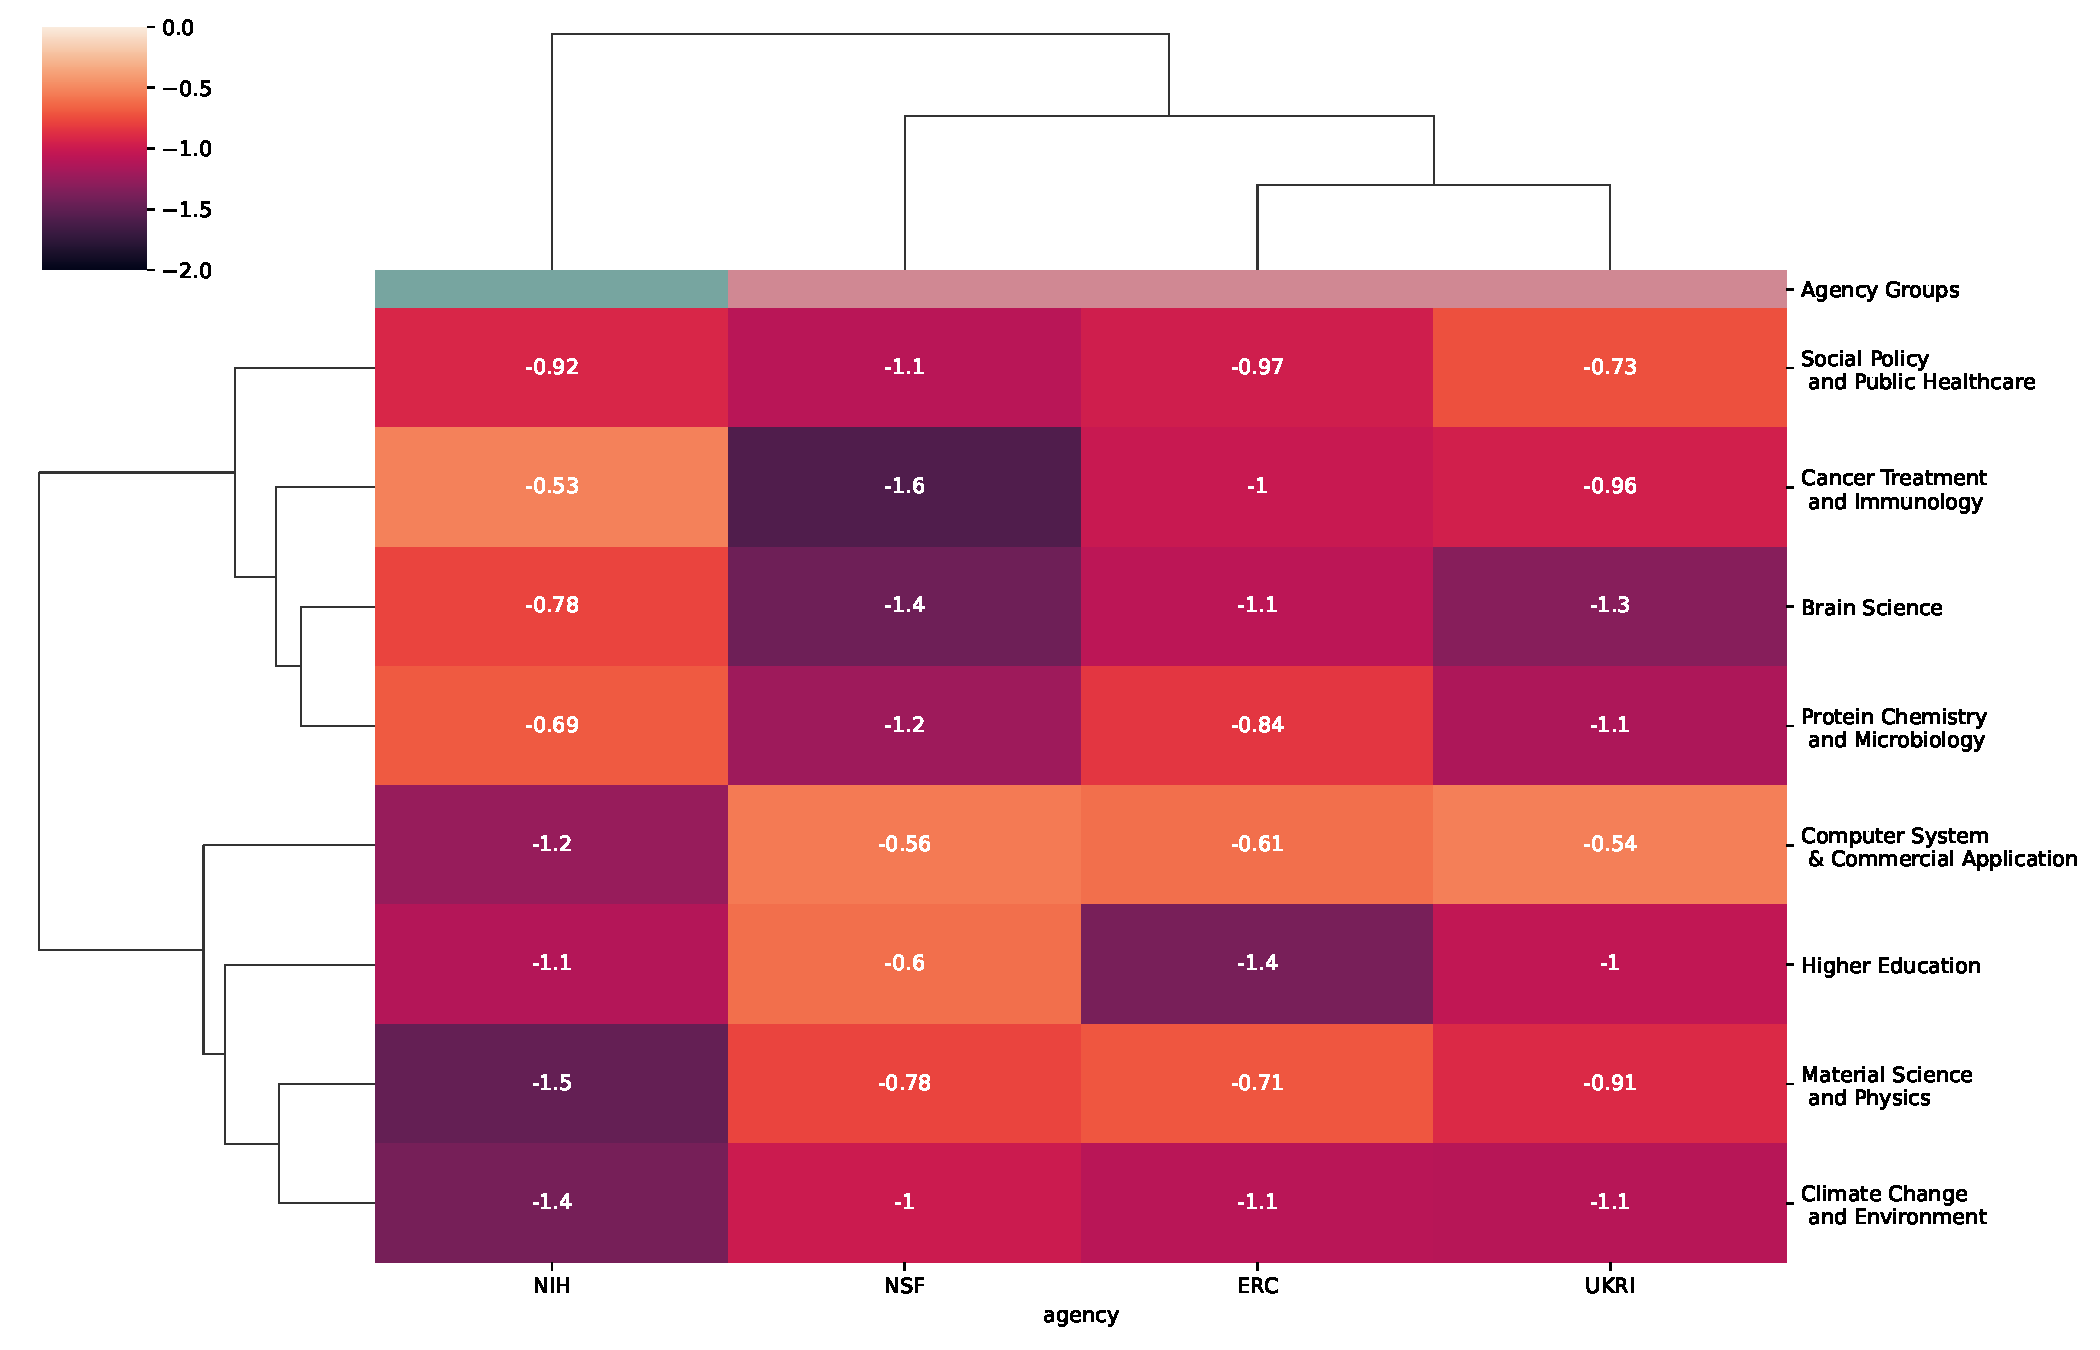
\includegraphics[width = 16cm, height = 9cm]{Code/img/heatmap_agency_topics.pdf}
    \caption[Heatmap between topic and agencies]{\textbf{Topics-Agencies Heatmap:} The heatmap between topics and four agencies. The colours inside the heatmap represent the base 10 log-scaled mean occurrence probabilities of topics. The darker is the colour, the fewer occurrence probabilities for the topic. The column and row dendrograms represent the results of hierarchical clustering on agencies and topics respectively. The two colours at the top heatmap represent different amount areas of daily funding amount: dark-green is the NIH group, dark-pink is the group of all other agencies.}
\end{figure}

For the group of all other agencies (Fig. 7A), the mean probabilities of topic ``Brain Science" that occur at the low-amount and medium-amount areas are low, but becoming larger at the high-amount area of the daily funding amount. For the topics ``Protein Chemistry and Microbiology" and ``Cancer Treatment and Immunology", they are also less probable of occurring at the low-amount area and increasingly likely to be at the areas of daily medium- and high-amount of funding, even though they have the lowest occurrence probabilities occurring in the group of all other agencies. For the ``Social Policy and Public Healthcare" topic, it is more likely to be funded at the range from 0 to 69.6 dollars and the range from 344.5 to 388.3 dollars, comparing with other intervals of the funding amount. The ``Climate Change and Environment" topic has a relatively high probability of occurrence between 193.7 and 203.1 dollars, at the highest ranges of the low-amount area. Except for the interval between 0 to 36.5 dollars, the probability of appearance of the topic ``Computer System \& Commercial Application" is evenly distributed. The funded projects related to ``Higher Education" are more probable to be funded at low-amount funding area than at the medium- and high-amount areas. For the topic ``Material Science and Physics", the projects in the group of all other agencies are more likely to be funded at the medium-amount area, compared to be at the low- and high-amount areas.

\begin{figure}[H]
    \centering
    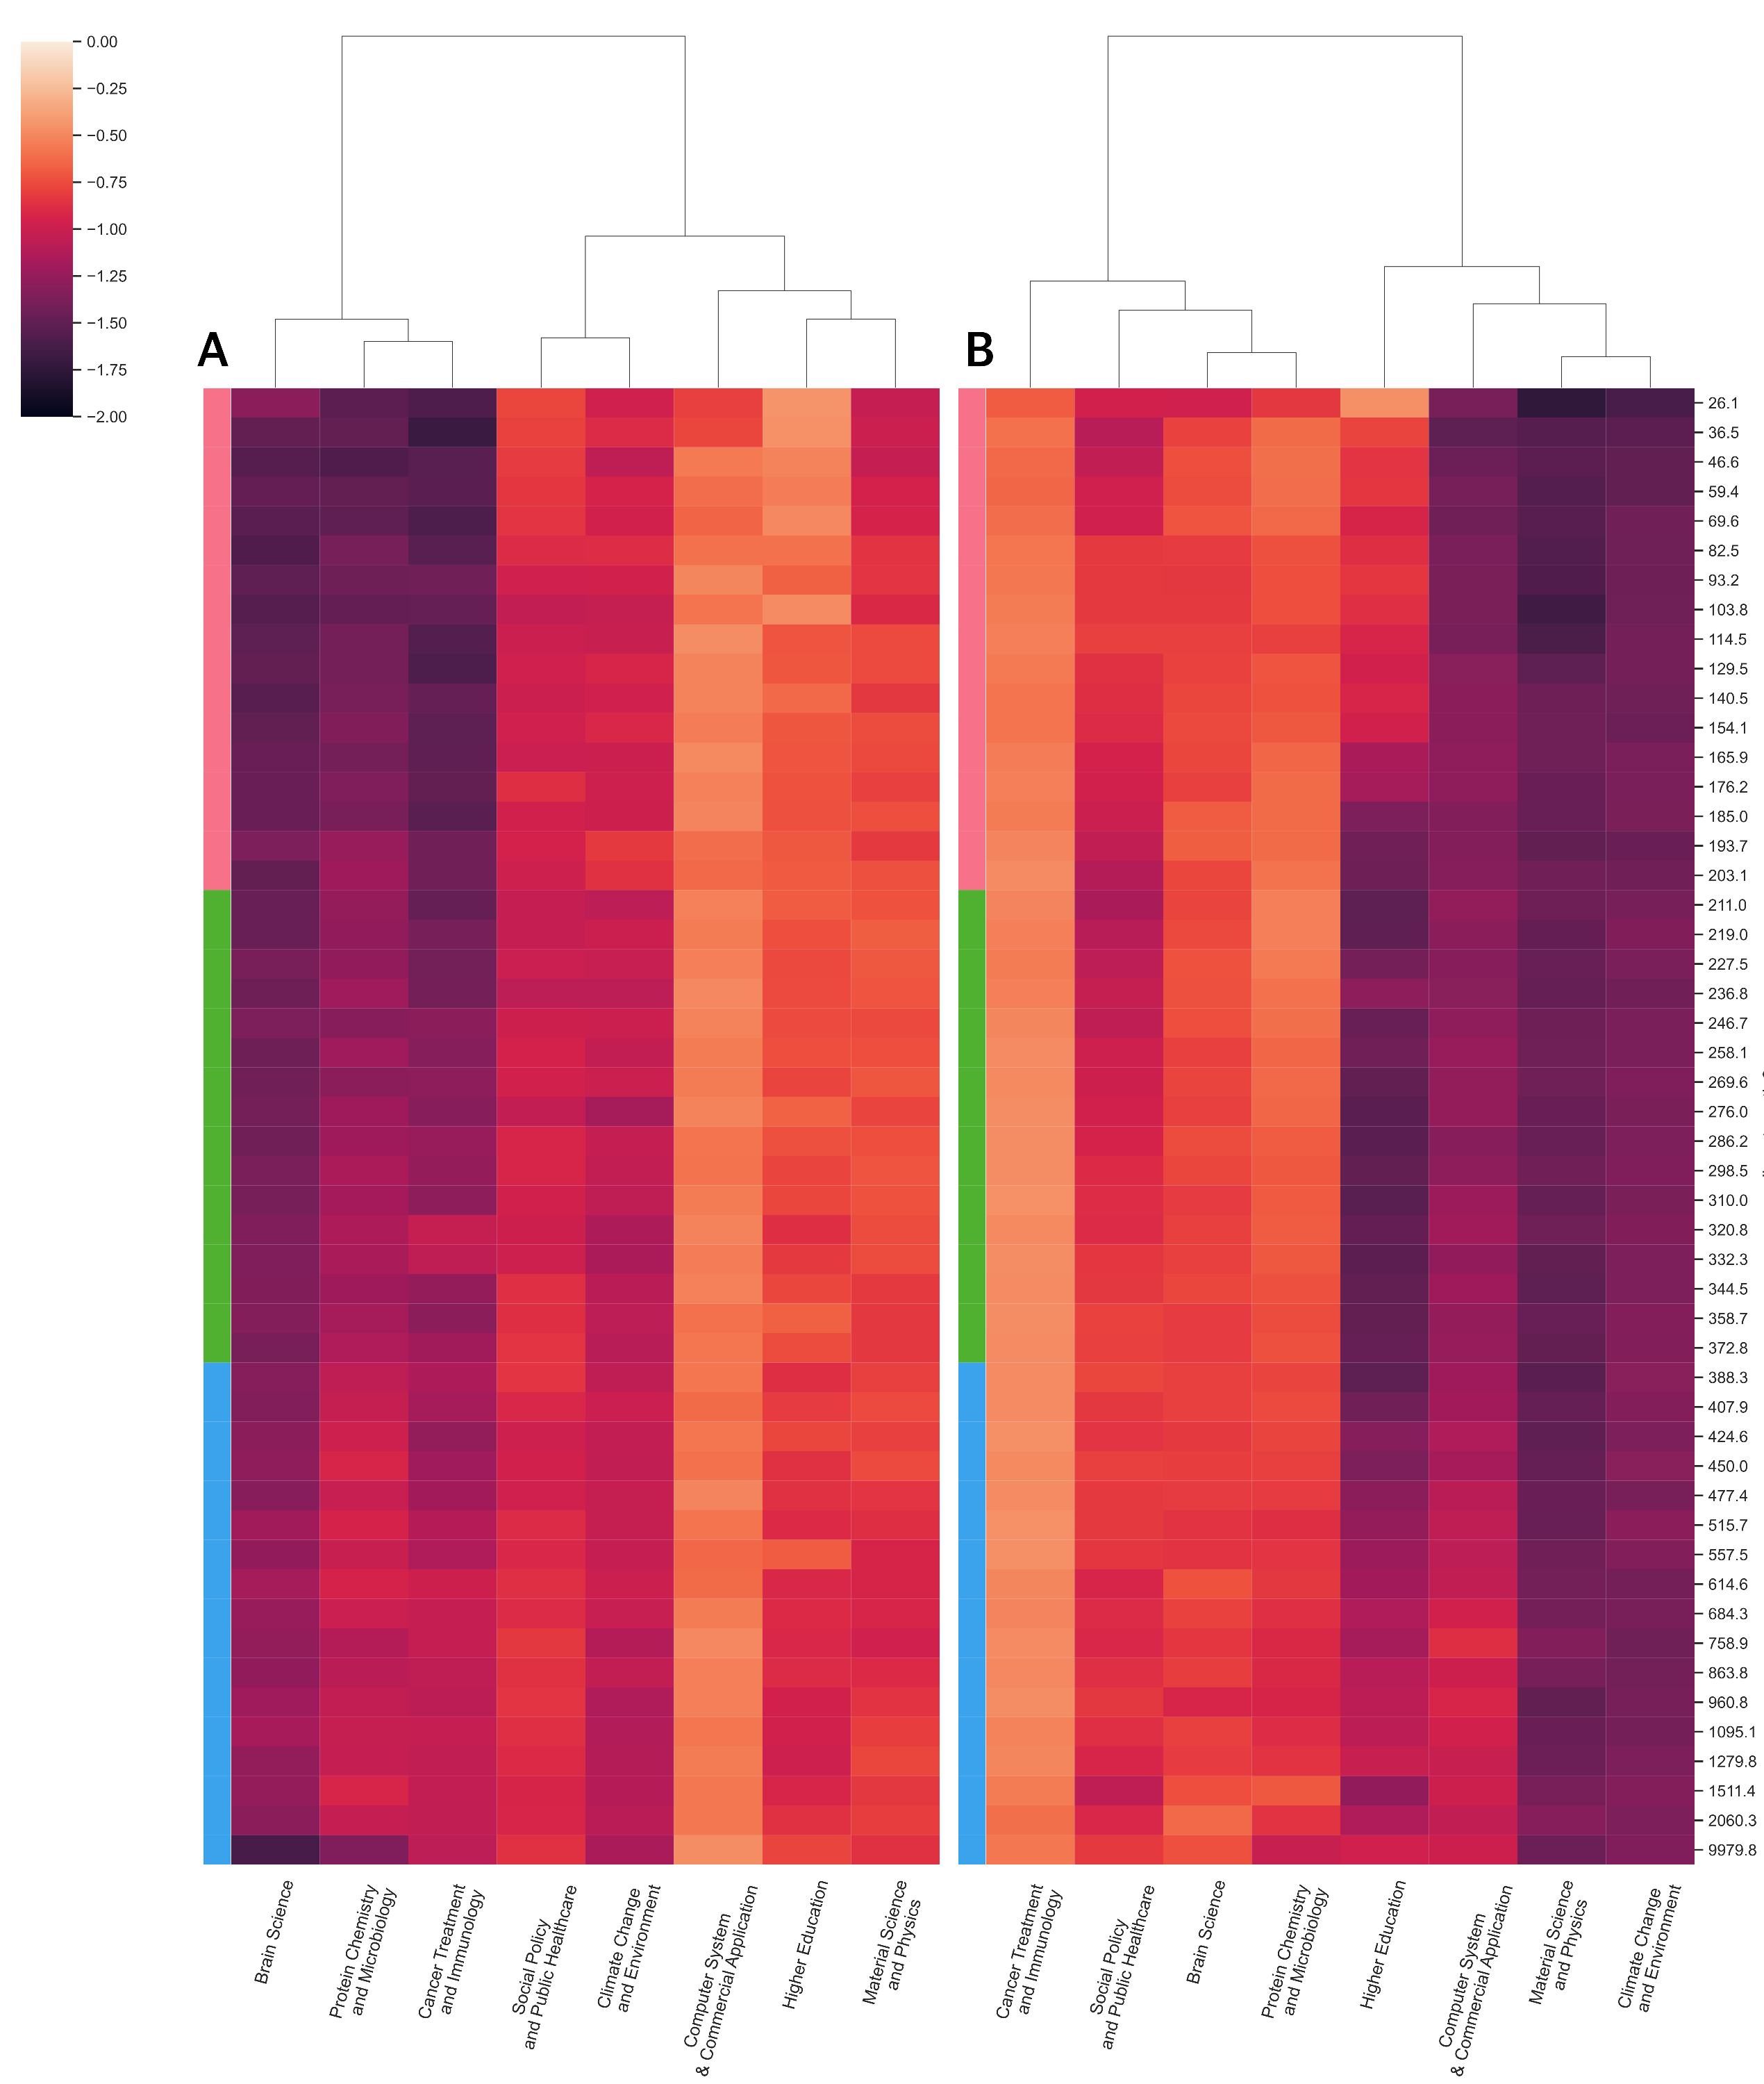
\includegraphics[width = 16cm, height = 21cm]{Code/img/heatmap_amount_topics.pdf}
    \caption[Heatmaps between topics and 50 intervals of discrete funding amount]{\textbf{Topics-Amount Heatmap:} The heatmap A and B gives the base 10 log-scaled mean occurrence probabilities of eight topics between 50 intervals of daily funding amount (see section 2.5) in NSF, ERC and UKRI agencies and in the NIH agency respectively. The vertical axis represents the discrete daily funding amount, the horizontal axis represents the agencies. Three colours on the left side of A and B describe three areas of the daily funding amount: Pink is the low-amount area, Green is the medium-amount area and Blue is the high-amount area. The column dendrogram gives the result of hierarchical clustering on topics.}
\end{figure}

For the NIH, a health-focused agency (Fig. 7B), topics ``Climate Change and Environment" and ``Material Science and Physics" have equal distributions but the lowest occurrence probabilities over three areas of daily funding agencies. The probability of occurrence of the ``Cancer Treatment and Immunology" topic is evenly distributed over the intervals of daily funding amount and, compared with other topics, is highest in NIH agency. There is an opposite trend that can be identified between the topics ``Computer System \& Commercial Application" and ``Higher Education". The projects related to the former topic is more probable to be funded at a high-amount funding area between 684.3 and 9979.8 dollars each day, whereas projects in NIH agency that are relevant to the latter topic are more likely to be funded at the low-amount area between 0 dollar and 154.1 dollars per day. Furthermore, the NIH funded projects related to ``Brain Science" have a higher probability of obtaining funding at ranges of 176.2--193.7 dollars and 1279.8--2060.3 dollars per day. The ``Protein Chemistry and Microbiology" appears with a higher probability at the range from 26.1 and 69.6 dollars and the range from \$203.1 to \$227.5 per day. Additionally, the topic ``Social Policy and Public Healthcare" is more likely to appear in some low intervals of daily funding amount at the low-amount and high-amount areas.

In general, the occurrence probabilities of two dominated topics (``Computer System \& Commercial Application" and ``Cancer Treatment and Immunology") in the NIH agency group and the group of all other agencies are both distributed evenly at the three areas of the daily funding amount. The probability of occurrence of these two topics increases over the intervals of daily funding amount if the two topics exchange groups with each other. In addition, in the group of all other agencies, with the unchanged distribution of the probability that the topic ``Computer System \& Commercial Application" occurs, the occurrence probabilities of ``Protein Chemistry and Microbiology" and ``Brain Science" topics rise with increasing daily funding amount.

\subsection{Prediction of Funding Amount}

\begin{figure}[H]
    \centering
    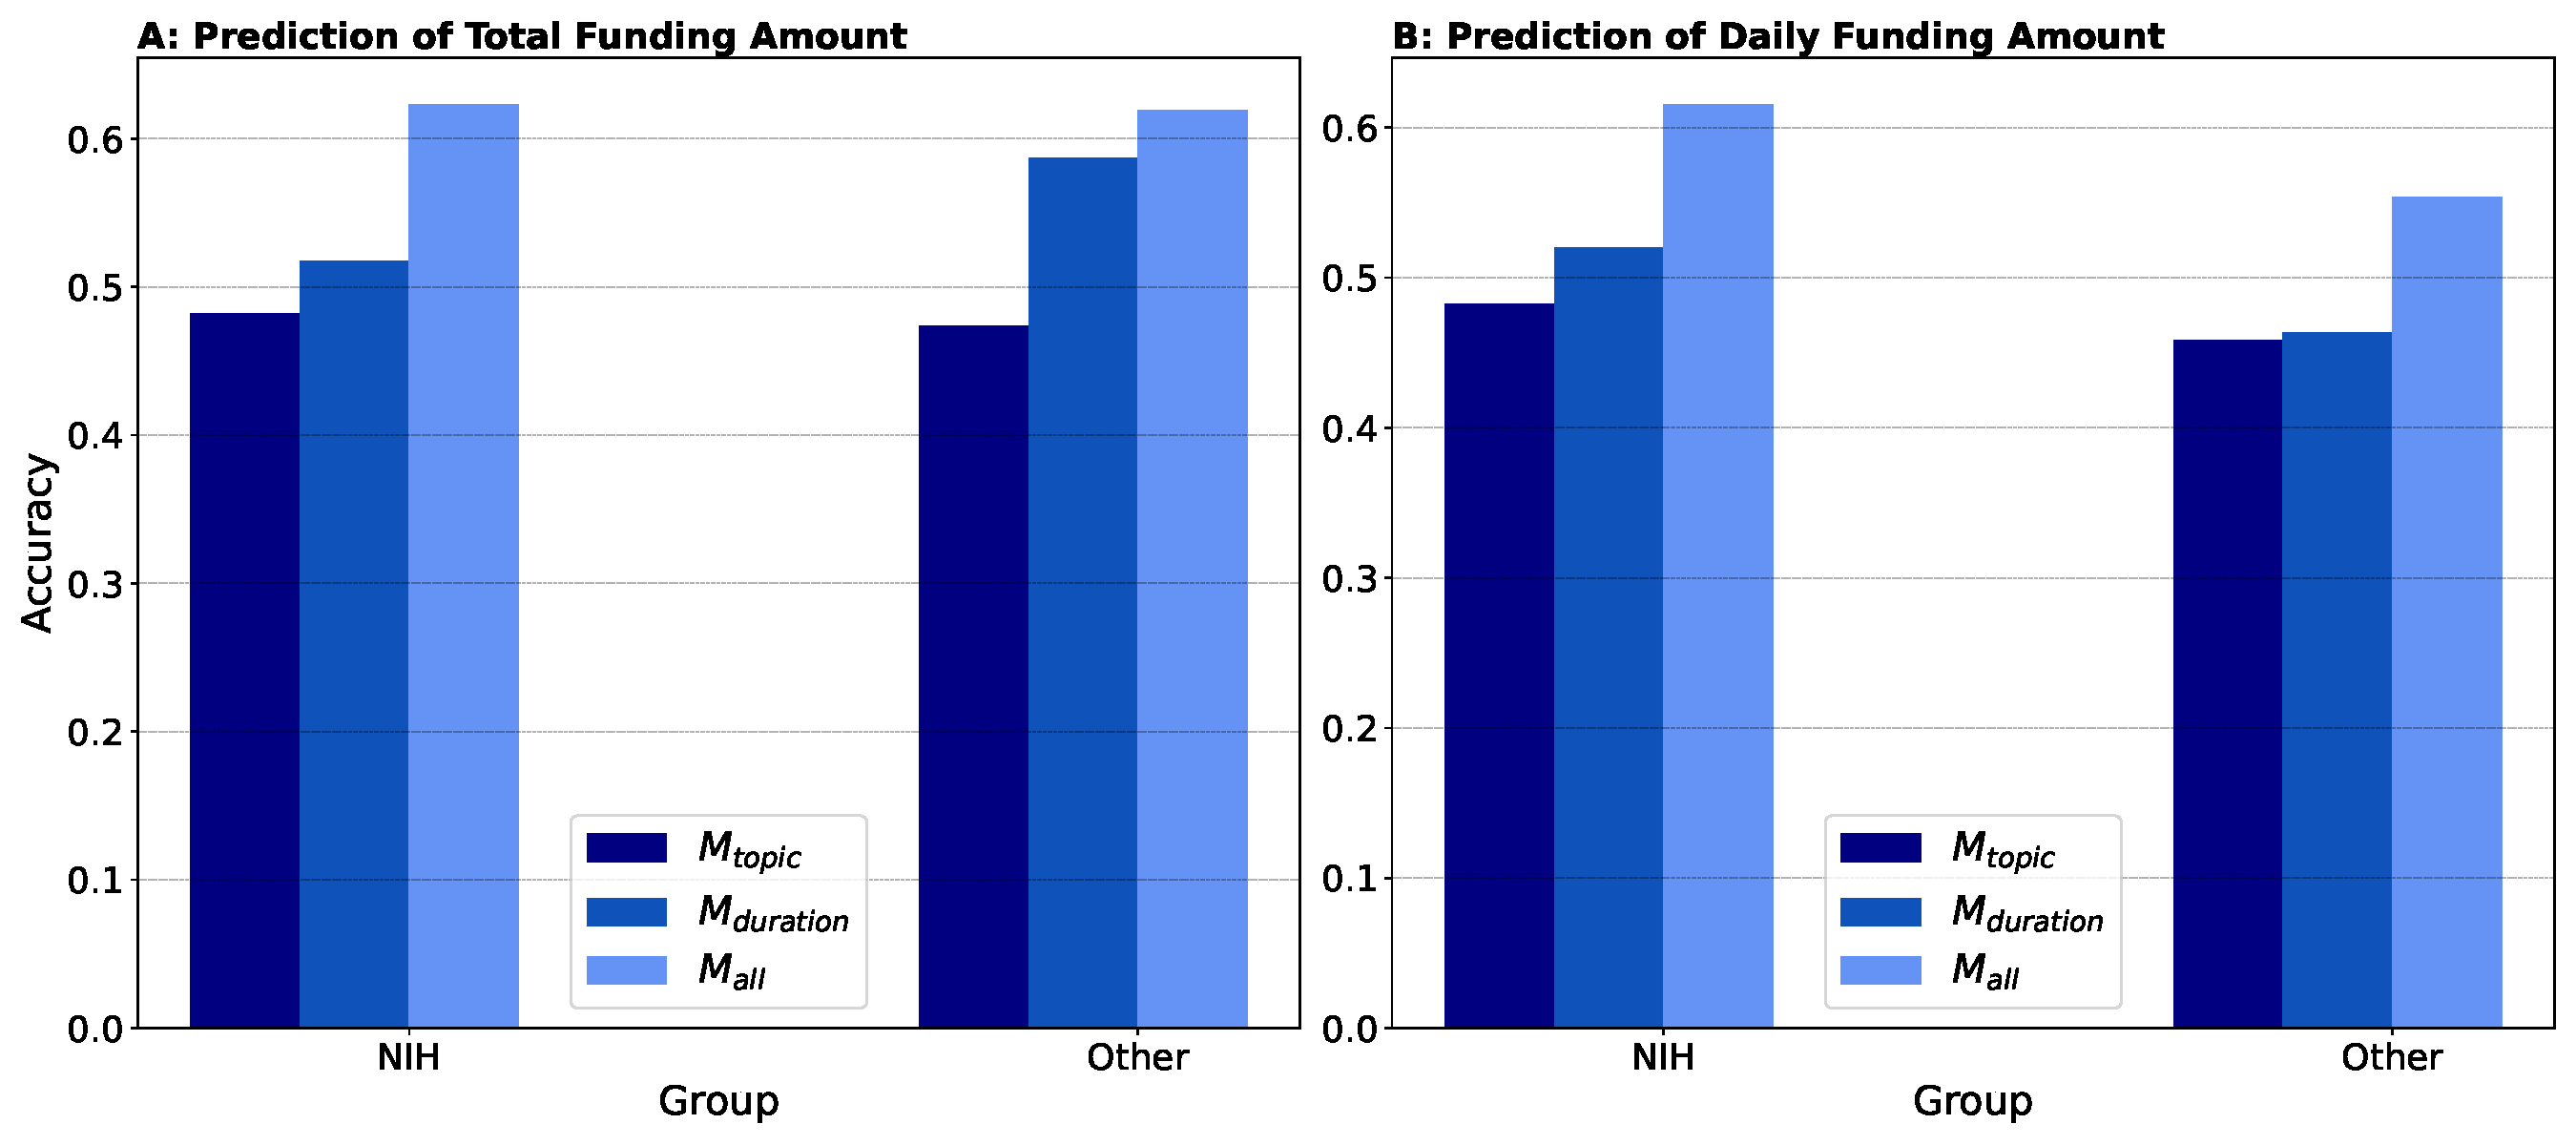
\includegraphics[width = 17cm, height = 8cm]{Code/img/accuracy_daily.pdf}
    \caption[The accuracy of prediction of funding amount using LightGBM]{\textbf{Prediction Accuracy:} The accuracy of prediction of the total and daily funding amount using LightGBM in NIH group and the group of all other agencies.}
\end{figure}

As predicting the total funding amount, the $M_{topic}$ in both the NIH group and all other agencies obtained the lowest accuracy, at approximately 0.482 and 0.474. Having only project duration as a feature, the accuracy of $M_{duration}$ in all other agencies is 0.587, 13.3\% higher than that of $M_{duration}$ in the NIH group. As combining all topic distributions and project durations together as predictors, both the accuracy of $M_{all}$ are beyond 0.6, boosting 20.4\% in the NIH group and 5.5\% in all other agencies compared with the accuracy of $M_{topic}$. When the prediction target is the daily funding amount, a different situation is seen in the group of all other agencies. The accuracy of $M_{duration}$ and $M_{all}$ in all other agencies decreases by 10.5\% and 8.5\% respectively, compared with that of corresponding models in the NIH group. However, regardless of whether the prediction target is either total or daily funding amount, the accuracy of prediction is improved in all groups with adding the topic distributions into predictors.
